\documentclass[12pt,a4paper]{article}

% incluyendo paquetes
\usepackage[utf8]{inputenc}
\usepackage[spanish]{babel}
\usepackage{milibreria}

\graphicspath{{C:/Users/HUAWEI/Pictures/imagesppt/}} %\incluye todos las imágenes de esa ruta
%\graphicspath{{D:/proyectos_latex/7mo_semestre/gestion_redes/informe_de_redes/main/images}}
\begin{document} % inicio  de documento 



\begin{titlepage}
    %\begin{tikzpicture}[overlay, remember picture]
    %    \fill[red] (10cm,-10cm) rectangle (5cm,-15cm);
    %\end{tikzpicture}
    
    \miRectangulo{-2cm}{-4cm}{2cm}{5cm}{rosado}
%   \miRectangulo{x     }{y }{x1    }{y1   }{color}
    
    \miRectangulo{-1.5cm}{-2cm}{-1.2cm}{23.5cm}{black} % 1
    \miRectangulo{-1.8cm}{23.5cm}{5.7cm}{23.2cm}{black} % 2
    \miRectangulo{5.025cm}{23.5cm}{5.33cm}{20cm}{black} % 3
    \miRectangulo{-2.7cm}{-1.7cm}{4.7cm}{-2cm}{black} % 4
    \miRectangulo{4.2cm}{-2cm}{4.5cm}{10cm}{black} % 5

    \begin{textblock}{100}(100,20)
        \begin{flushright}
        {\huge{\textbf{Universidad Nacional del Altiplano}}}\\
        {\normalsize{\textbf{Educando mentes, Cambiando el mundo}}}
        \end{flushright}
        
    \end{textblock}
    
    \begin{tikzpicture}[remember picture, overlay]
        \node at (current page.north west) [anchor=north west, xshift=120mm, yshift=-47mm] {\includegraphics[width=0.45\textwidth]{\logoright}};
    \end{tikzpicture}
    \begin{textblock}{100}(100,130)
        \begin{flushright}
            {\Large{\textbf{Facultad de Ingeniería Mecánica Eléctrica,
                    Electrónica y Sistemas}}}\\[10pt]
            {\large{\textbf{Escuela Profesional de Ingeniería\\ de Sistemas}}}
        \end{flushright}
    \end{textblock}

    \begin{textblock}{200}(10,163)
        \begin{center}
            
            %\textcolor{azul}{\rule{\linewidth}{0.80mm}}
            % titulo del articulo
            {\LARGE {\textbf{ Tipos de Auditoria }}} \par

            \textcolor{azul}{\rule{0.5\linewidth}{0.80mm}} \par
            \vspace{8mm}
            {\large{\textbf{ Auditoría en sistemas }}} \\[10pt]
            {\large{\textbf{\textcolor{azul}{ing. TICONA YANQUI FIDEL ERNESTO }}}} \\[20pt]
            {\large{\textbf{estudiante}}}\\[10pt]
            {\large{\textbf{$\looparrowright$   Larota Pilco David Brahyan  $\looparrowleft$ }}}\\[5pt]
            %{\large{\textbf{$\looparrowright$    Quispe Calcina Royer $\looparrowleft$ }}}\\[5pt]
            %{\large{\textbf{$\looparrowright$    Rojas Alejo Bruno $\looparrowleft$ }}}\\[5pt]
            %{\large{\textbf{$\looparrowright$  $\mathfrak{David\ Brahyan\ Larota\ Pilco}$   $\looparrowleft$ }}}\\[20pt]
            \today

        \end{center}
    \end{textblock}
\end{titlepage}
%//--------------------------------------
%@article{prueba,
%  title={prueba del documento lenguaje Latex},
%  author={Autor},
%  journal={https://www.overleaf.com/},
%  volume={13},
%  number={36},
%  pages={34--36},
%  year={2022}
%}
%
%
%\begin{figure}[h]
%    \centering
%    \includegraphics[width=0.5\textwidth]{images/medicion_con_tacometro.png}
%    \caption{se realizo la medición con el tacómetro} 
%\end{figure}
%
%\begin{tabular}{ l c l }
%Tipo  			& = & 	GL-90L-4B5 \\
%Ip              & = &	55 \\
%Cos  $\varphi$    & = &  	  0.78 \\
%Voltaje         & = &	 230/400V \\
%Potencia	    & = &	2HP \\
%Intensidad    	& = & 	6.1/3.5 \\
%Frecuencia  	& = & 	60HZ \\
%Rpm     		& = &	1680 
%\end{tabular} % incluyendo la caratula
%\tableofcontents % índice automático
\pagestyle{fancy} \mystyle \newpage % Aplicar el estilo de encabezado y pie de página
% inicio del documento  

\section{Resumen}
Los diferentes tipos de auditorías desempeñan roles específicos en la evaluación y mejora de las organizaciones. La auditoría financiera se centra en la revisión de los estados financieros y la gestión administrativa para garantizar la conformidad con los estándares contables y financieros. Por otro lado, la auditoría operativa se enfoca en mejorar la eficiencia y efectividad de los procesos operativos de una empresa, buscando identificar áreas de mejora para aumentar la productividad y la calidad. La auditoría informática se ocupa de evaluar los sistemas informáticos y la seguridad de la información para proteger los activos digitales contra posibles amenazas. Finalmente, la auditoría de gestión evalúa los procesos de gestión y dirección de una organización para garantizar el cumplimiento de los objetivos estratégicos y la eficiencia operativa. Cada tipo de auditoría proporciona una perspectiva única que contribuye a la mejora continua y al éxito global de una organización.

\newpage
\section{Definicion de Auditoria}
\DleftRule[\cite{definicion}.]{Según  \citeauthor{definicion}\ Una auditoría es una revisión sistemática de una actividad o situación para evaluar el cumplimiento de las reglas o criterios objetivos a los que estas deben someterse }
Su objetivo principal es verificar la veracidad, integridad y precisión de la información, así como garantizar el cumplimiento de normativas y estándares establecidos. La auditoría puede aplicarse en diversos contextos, incluyendo aspectos financieros, contables, operativos, ambientales, y de calidad, entre otros.

\begin{figure}[!htb]
    \centering
    \caption{Auditoria} 

    
\includegraphics[width=0.5\textwidth]{images/audit_online_3.jpg}
    \par
    \textit{imagen descargada de:} \cite{img_auditoria}

\end{figure}


\newpage
\section{Auditoría Financiera} 
Se enfoca en verificar la precisión de los registros financieros y en determinar si la organización ha cumplido con todas las leyes y regulaciones relacionadas
\cite{audit_financiera}.

\subsection*{Ejemplo}
Supongamos que una empresa de fabricación de muebles contrata a una firma de auditoría para realizar una auditoría financiera. Durante el proceso, los auditores revisarán los estados financieros de la empresa, incluyendo el balance general, el estado de resultados y el flujo de efectivo. Examinarán las transacciones pasadas y actuales, verificarán la exactitud de los registros contables, evaluarán el cumplimiento de las normas contables y las leyes fiscales, y buscarán posibles errores o fraudes. Al finalizar, presentarán un informe detallado que refleje sus hallazgos y recomendaciones para mejorar los controles internos y la precisión de la información financiera.
\begin{figure}[!htb]
    \centering
    \caption{Auditoria Financiera} 

    
\includegraphics[width=0.3\textwidth]{images/audi_financiera.jpg}
    \par
    \textit{imagen descargada de:} \cite{fig_financiera}.

\end{figure}


\newpage
\section{Auditoría de Cumplimiento} 
La auditoría de cumplimiento se enfoca en evaluar si una empresa cumple con las leyes, regulaciones, políticas internas y procedimientos establecidos. Este tipo de auditoría se centra en verificar si la organización está operando de acuerdo con los requisitos legales y normativos aplicables a su industria y actividades comerciales.
\cite{audit_cumplimiento}.

\subsection*{Ejemplo}
Imaginemos una compañía de servicios financieros que solicita una auditoría de cumplimiento. Durante el proceso, los auditores revisarán minuciosamente las prácticas y políticas de la empresa para asegurarse de que cumplan con todas las regulaciones financieras y normativas, como la Ley de Privacidad de la Información Financiera (GLBA) o la Ley Sarbanes-Oxley (SOX). Examinarán los controles internos, las prácticas de gestión de riesgos, los procedimientos de cumplimiento y los registros de transacciones para determinar si la empresa está cumpliendo con todas las leyes y regulaciones pertinentes. Al finalizar, emitirán un informe detallado con sus hallazgos y recomendaciones para abordar cualquier deficiencia o área de mejora identificada.


\begin{figure}[!htb]
    \centering
    \caption{Auditoria de Cumplimiento} 

    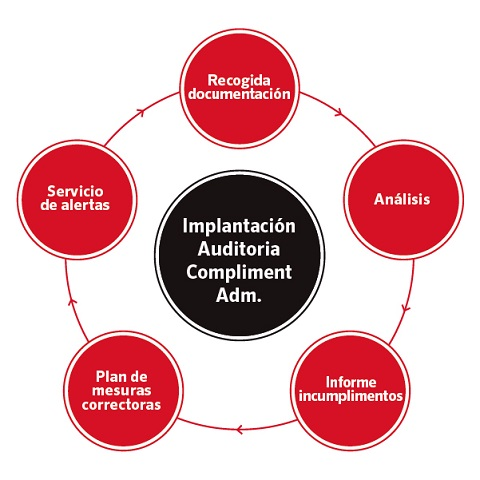
\includegraphics[width=0.3\textwidth]{images/fig_cumplimiento.jpg}
    \par
    \textit{imagen descargada de:} \cite{fig_cumplimiento}.

\end{figure}


\newpage
\section{Auditoría Operativa} 
La auditoría operativa es un proceso de revisión y evaluación de los procesos operativos de una organización para identificar oportunidades de mejora, eficiencia y eficacia en sus actividades. A diferencia de la auditoría financiera, que se centra en los aspectos contables y financieros, la auditoría operativa se enfoca en áreas como la gestión de recursos humanos, la gestión de la cadena de suministro, la producción, las ventas y el servicio al cliente
\cite{audit_operativa}.

\subsection*{Ejemplo}
Imaginemos una cadena de restaurantes que solicita una auditoría operativa. Durante el proceso, los auditores examinarán los procesos de preparación de alimentos, el servicio al cliente, la gestión de inventario y la administración de recursos humanos. Evaluarán la eficiencia de cada proceso, identificarán posibles cuellos de botella, analizarán los costos operativos y buscarán oportunidades para mejorar la productividad y la calidad. Por ejemplo, podrían recomendar la implementación de un nuevo sistema de gestión de inventario para reducir el desperdicio de alimentos o la optimización de los horarios de personal para aumentar la eficiencia en horas pico.

\begin{figure}[!htb]
    \centering
    \caption{Auditoria Operativa} 

    
\includegraphics[width=0.3\textwidth]{images/fig_operativa.jpg}
    \par
    \textit{imagen descargada de:} \cite{fig_operativa}.

\end{figure}

\newpage
\section{Auditoría de Información}
La auditoría informática, también conocida como auditoría de sistemas de información o auditoría de tecnología de la información (TI), se enfoca en evaluar los sistemas informáticos, la infraestructura de tecnología de la información y los controles de seguridad de una organización. El objetivo principal de esta auditoría es garantizar la integridad, confidencialidad y disponibilidad de la información, así como identificar y mitigar riesgos relacionados con la tecnología.
\cite{audit_sofware}

\subsection*{Ejemplo}
Supongamos que una empresa de servicios financieros solicita una auditoría informática. Durante el proceso, los auditores revisarán los sistemas informáticos de la empresa, incluyendo redes, servidores, bases de datos y aplicaciones. Evaluarán los controles de seguridad, como el acceso a los datos, la protección contra malware y la gestión de parches de seguridad. Además, realizarán pruebas de penetración para identificar vulnerabilidades en la infraestructura y evaluar la preparación de la empresa para enfrentar posibles ciberataques. Al finalizar, presentarán un informe detallado con recomendaciones para mejorar la seguridad de la información y garantizar el cumplimiento de las regulaciones de privacidad y seguridad de datos.

\begin{figure}[!htb]
    \centering
    \caption{Auditoria de Información} 

    
\includegraphics[width=0.3\textwidth]{images/fig_sistemas.jpg}
    \par
    \textit{imagen descargada de:} \cite{fig_software}.

\end{figure}

\newpage
\section{Auditoría de Gestión o de Desempeño} 
La auditoría de gestión, también conocida como auditoría administrativa o de gestión empresarial, se enfoca en evaluar los procesos de gestión y dirección de una organización. El objetivo principal es identificar áreas de mejora en la eficiencia operativa, la efectividad de las políticas y procedimientos, y el logro de los objetivos estratégicos de la empresa.
\cite{audit_gestion}
\subsection*{Ejemplo}
Supongamos que una empresa de fabricación de automóviles solicita una auditoría de gestión. Durante el proceso, los auditores revisarán los procesos de producción, distribución, marketing, recursos humanos y finanzas. Evaluarán la eficacia de las políticas y procedimientos en cada área funcional, analizarán los indicadores clave de rendimiento (KPIs) para medir el desempeño y compararán los resultados con los objetivos estratégicos de la empresa. Por ejemplo, podrían examinar la eficiencia de la cadena de suministro para identificar posibles retrasos en la entrega de componentes, revisar la efectividad de las campañas de marketing para aumentar las ventas, o evaluar la rotación de personal y la satisfacción laboral para mejorar la retención de empleados.


\begin{comment}
\newpage
\section{Auditoría Forense} 
Este tipo de auditoría se realiza para investigar fraudes posibles o reales en una empresa.

\newpage
\section{Auditoría Interna} 
Es realizada por personal interno de la empresa para identificar fortalezas y debilidades y sugerir áreas de mejora.

\newpage
\section{Auditoría Externa} 
Es realizada por una firma de auditoría independiente, normalmente para propósitos de informes anuales o para cumplir con regulaciones legales o gubernamentales.

\newpage
\section{Auditoría Fiscal} 
Se verifica la exactitud de los informes fiscales presentados por una empresa o un individuo.
\end{comment}

\newpage
\section{Referencias}
\bibliographystyle{apacite}
\bibliography{referencias.bib}


\end{document}